Capgemini France est composé de vingt-sept sites répartis dans toute la France et accueillant 21 110 collaborateurs générant un chiffre d'affaires de 2 193.9 millions d'euros.

\begin{figure}[!h]
    \centering
        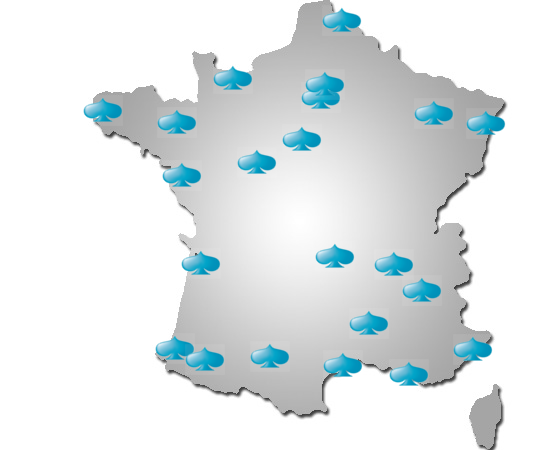
\includegraphics[width=10cm]{img/capgeminiFrance.png}
        \caption{Capgemini France}
        \label{fig:capgeminiFrance}
\end{figure}

\subsection{Capgemini Ouest}

 La filiale Capgemini Ouest constituée des sites de Nantes, Rennes, Bordeaux, Tours, Orléans, Brest, Rouen et Caen est implantée depuis 1974. Capgemini offre les meilleures ressources au meilleur endroit pour le meilleur prix grâce au Collaborative Business Experience et au modèle Rightshore. Capgemini Ouest se distingue particulièrement dans les secteurs du service public, de l'assurance et des Télécoms.
 
\begin{figure}[!h]
    \centering
        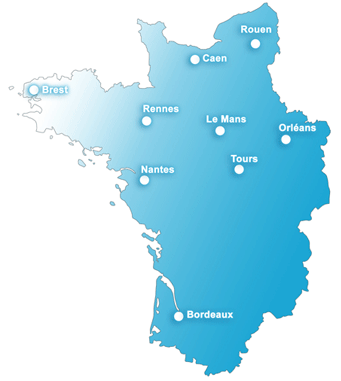
\includegraphics[width=10cm]{img/capgeminiOuest.png}
        \caption{Capgemini Ouest}
        \label{fig:capgeminiOuest}
\end{figure}

\clearpage
\subsection{Capgemini Nantes}

Capgemini Nantes s'occupe principalement de banque et d'assurance bien qu'un pôle, l'ADM, soit spécialisé dans l'accompagnement des entreprises de service comme la Poste ou la SNCF. La SNCF est d'ailleurs au centre de plusieurs centres de service dédiés.

\begin{figure}[!h]
    \centering
        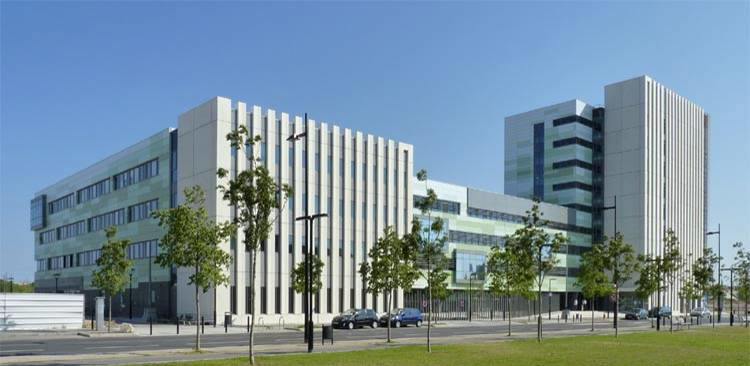
\includegraphics[width=10cm]{img/capgeminiNantes.png}
        \caption{Capgemini Nantes}
        \label{fig:capgeminiNantes}
\end{figure}

Suite à une récupération de marché en 2013, le service Distribution a fusionné avec un autre service (Transporteur) pour donner naissance au service Distribution/Transporteur dont la seule source d'activité est la SNCF.